\documentclass[a4paper, 12pt]{report}
%================================================================
\usepackage{verbatim, fancyhdr, theorem, dsfont, color,
            amsmath, amsfonts, amssymb,
            hyperref,epsfig, graphicx, setspace}
\usepackage{graphics}
\usepackage[margins]{trackchanges}
% to insert pdf sous la forme
% \includepdf[pages=-]{../CoherePart_CR1nov2012/rapportCoherence.pdf}
%\usepackage{pdfpages}
%============================================
 \textheight 21cm
% \doublespace
%  \oddsidemargin -0.5cm
% \evensidemargin +1.5cm
%  \textwidth 17cm
% \topmargin 0cm
%============================================
% Figures
%============================================
\newcommand{\figsstit}[2]{
\begin{figure}[hbtp]
\centerline{
    \hbox{ \epsfig{figure={#1}, scale=#2} }
}
\end{figure}}
%============================================
\newcommand{\figscale}[4]{
\begin{figure}[hbtp]
\centerline{
    \hbox{ \includegraphics[scale=#4]{#1} }
}
\begin{center}
\parbox{12	 cm}
{
    \caption{\protect\small\it  {#2}}
    \label {#3}
}
\end{center}

\end{figure}}

%%============================================
%\newcommand{\figsstit}[2]{
%\begin{figure}[hbtp]
%\centerline{
%    \hbox{ \includegraphics{figure={#1}, scale=#2} }
%}
%\end{figure}}
%

%==============================================
\newcommand{\prob}[1]{\mathds{P}\left( #1 \right)}
\newcommand{\esp}[1]{\mathds{E}\left[ #1 \right]}
\newcommand{\var}[1]{\mathrm{var}\left( #1 \right)}
\newcommand{\cov}[1]{\mathrm{cov}\left( #1 \right)}
\newcommand{\diag}[1]{\mathrm{diag}\left( #1 \right)}
\newcommand{\trace}[1]{\mathrm{trace}\left( #1 \right)}
\newcommand{\card}[1]{\left| #1 \right|}
\newcommand{\myemph}[1]{\emph{\color{red}#1}}


 \newcommand{\benoit}[1]{\marginpar{\color{red}\footnotesize{BENOIT:}
                \color{red}\footnotesize{ #1}}}

 \newcommand{\momo}[1]{\marginpar{\color{blue}\footnotesize{MOMO:}
                \color{blue}\footnotesize{ #1}}}
%%============================================================================
%\def\thesection{\arabic{section}.}
%\def\thesubsection{\arabic{section}.\arabic{subsection}}
%\def\thesubsubsection{\arabic{section}.\arabic{subsection}.\arabic{subsubsection}}
%\def\thefigure{\arabic{figure}}
%\def\theequation{\arabic{equation}}
%\def\theexercice{\arabic{exercice}}
%\def\theexample{\arabic{example}}
%\def\theproof{\arabic{proof}}

%===============================================
\newtheorem{property}{Properties}
\newtheorem{remark}{Remark}
\newtheorem{theorem}{Theorem - \thetheoreme}
\newtheorem{definition}{Definition - \thedefinision}
\newtheorem{example}{Example}
\newtheorem{lemme}{Lemme - \thelemme}
\newtheorem{proof}{Proof - \theproof}
\newenvironment{TAB}{\begin{table}[[hbt] \center \leavevmode}{\end{table}}
%%=========== LOGO/Head/Foot par PAGE ========
%\pagestyle{fancy}
% \lhead[]{}
% \chead[]{}
% \rhead[]{\includegraphics[scale=0.1]{\DIRLOGO/logo_telecomparis}}
% \lfoot[]{\thechapter}
% \cfoot[]{}
% \rfoot[]{\thepage}

%%============================================================================
%\newcounter{auxiliaire}
%%%%%%%% comment
%\setcounter{auxiliaire}{\theenumi}
%\end{enumerate}
% TEXTE
%\begin{enumerate}
%\setcounter{enumi}{\theauxiliaire}
%%============================================================================
%\renewcommand\arraystretch{1.6}

\def\ua{\underline a}
\def\ub{\underline b}
\def\uB{\underline B}
\def\uH{\underline H}
\def\ur{\underline r}
\def\us{\underline s}
\def\ux{\underline x}
\def\uX{\underline X}
\def\uZ{\underline Z}
\def\utheta{\underline \theta}
\def\hat{\widehat}

\def\MSC{\mathrm{MSC}}
\def\SNR{\mathrm{SNR}}
\def\iSNR{\mathrm{SNR}^{-1}}

\def\degree{$^{\circ}$}

\def\ut{{u}}
\def\rf{{r}}

%============== colors ========================
\definecolor{enstrouge}{RGB}{212,65,84}
\definecolor{lightorange}{RGB}{235,226,52}
\definecolor{greennoise}{RGB}{243,42,255}
\definecolor{lightred}{RGB}{255,181,183}
\definecolor{light-grey}{rgb}{0.95,0.95,0.95}
\definecolor{peach}{rgb}{0.98,0.49,0.25}
\definecolor{burntorange}{rgb}{0.79,0.37,0}
\definecolor{light-yellow}{rgb}{1,1,0.92}

\definecolor{light-green}{RGB}{231,255,145}
\definecolor{enstorange}{RGB}{255,214,10}
\definecolor{enstrouge}{RGB}{212,65,84}
\definecolor{grey}{RGB}{204,204,204}
\definecolor{blue}{RGB}{0,0,255}
\definecolor{almost-black}{RGB}{100,100,100}
\definecolor{violet}{rgb}{0.4,0,0.4}
\definecolor{cyan}{RGB}{0,255,255}
\definecolor{magenta}{RGB}{243,42,255}

\def\degree{^{\circ}}
\def\simiid{\stackrel{\mathrm{i.i.d.}}{\sim}}
\def\MSC{\mathrm{MSC}}%{\MSC}}
\def\hMSC{\widehat{\MSC}}%{\MSC}}


 \def\programsfullprocess{fullprocess/}
 \def\programsToolbox{fullprocess/ZZtoolbox/}
 \def\programspierrick{fullprocess/ZZtoolbox/00Pierrick/}



\graphicspath{{figures/}}
%============================================
\begin{document}
 \sloppy
%  \nocite{*}
 \bibliographystyle{plain}
\tableofcontents

\chapter{Utilisation}

\section{Introduction}
This document describes the version lite of the estimation process. The inputs are the two signals of any length which represent the signals from the system under test (SUT) and the system of reference (SREF). It performs the ratio between the auto-spectrum of SUT divided by the cross-spectrum of SREF on a given list of frequencies. The length of the list of frequencies is denoted $N$.

The ratio denoted $R_{\sup}$ is not corrected by the response of the SREF, nor the response of the noise reduction system.

The computation needs the description of the filter bank which is provided by a Matlab structure. That can be removed. The call function is

{\tiny\verbatiminput{estimSUTlitesynopsis.m}}


The outputs are the 
\begin{itemize}
\item
list of the $N$ values of  $R_{\sup}$ averaged on the full signals
\item
list of the $N$ values of  STDs of the module and the phase of $R_{\sup}$ performed on the full signals,
\item
list of the $N$ count number over the MSC threshold.                                                                                                                                                                                                                                                                                                                                                                                                                                                                                                                                                                                                                                                                                                                                                                                                                                                                                                                                                                                                                                                                                                                                                                                                                                                                                                                                                                                                                                                                                                                                                                                         
\end{itemize}

To play you can use the program { \tt estimationwithFBlite.m}


 \newpage
\section{Examples}


\subsection{Example 1}
The figure corresponds to the randomly chosen following days on station 1:

\begin{tabular}{cc}
 \begin{minipage}{0.35\textwidth}
 days:\\
 {\tt   2015/06/05-06}\\
 {\tt   2015/06/11-12}  \\
 {\tt   2015/07/01-02}  \\
 {\tt   2015/07/13-14}  \\
 {\tt   2015/08/03-04}  \\
 {\tt   2015/08/07-08}  \\
 {\tt   2015/08/09-10}  \\
 {\tt   2015/08/19-20}  \\
 {\tt   2015/09/29-30}  \\
 {\tt   2015/10/25-26}  
\end{minipage}
&
 \begin{minipage}{0.35\textwidth}
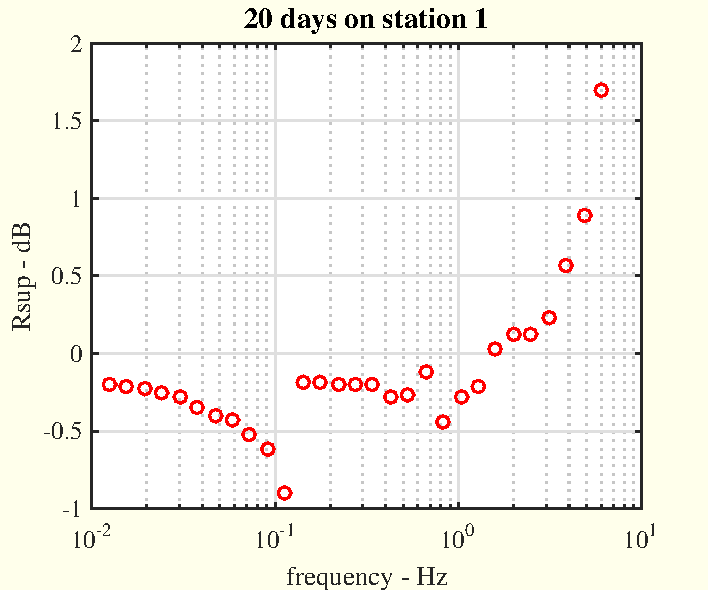
\includegraphics[scale=0.8]{example1onstation1.pdf}
\end{minipage}
\end{tabular}
 
 
\subsection{Example 2}
The figure corresponds to the randomly chosen following days on station 1:
\begin{tabular}{cc}
 \begin{minipage}{0.35\textwidth}
 days:\\
 {tt 2015/07/11-12 }\\
{tt 2015/07/13-14 }\\
{tt 2015/07/21-22 }\\
{tt 2015/07/27-28 }\\
{tt 2015/08/23-24 }\\
{tt 2015/09/07-08 }\\
{tt 2015/09/11-12 }\\
{tt 2015/09/15-16 }\\
{tt 2015/10/03-04 }\\
{tt 2015/10/21-22 }
\end{minipage}
&
 \begin{minipage}{0.35\textwidth}
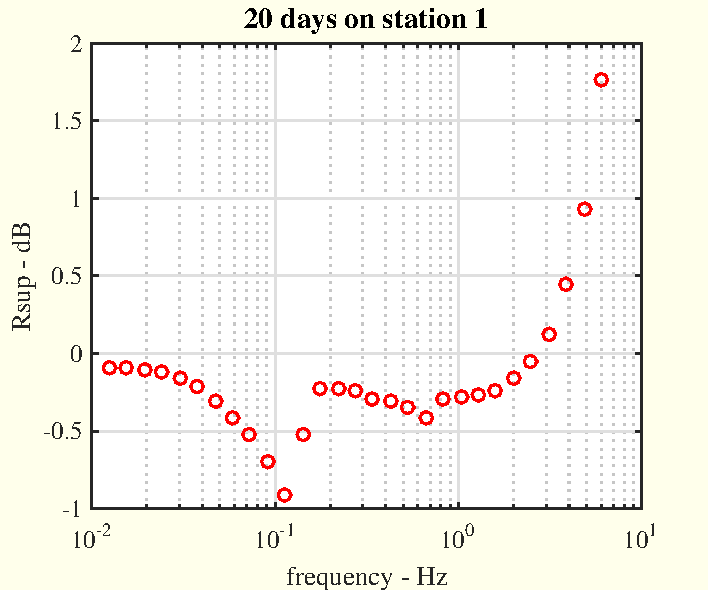
\includegraphics[scale=0.8]{example2onstation1.pdf}
\end{minipage}
\end{tabular}

\subsection{Example 3}
 The figure \ref{fig:example3onstation1} corresponds to $50$ randomly chosen days on station 1.  Because we  only save just what we need, the processing time (in Matlab) is only of $400$ seconds.

\figscale{example3onstation1.pdf}
{The blue points are the sequence of selected frequencies.}
{fig:example3onstation1}{0.8}

\chapter{Codes}
\section{Main program}
{\tiny\verbatiminput{../liteprocess/estimationwithFBlite.m}}

\section{Main function}
{\tiny\verbatiminput{../liteprocess/estimSUTlite.m}}

\end{document}




